\documentclass{article}
\usepackage{amsmath}
\usepackage{mathtools}
\usepackage{graphicx}% Include figure files
\usepackage{bm}% bold math
\usepackage{verbatim}
\usepackage{color}


\newcommand{\warning}[1]{{\textsf{{\textcolor{red}{{[#1]}{}}}}}}
\let\vec\mathbf

\begin{document}

\title{A cumulant analysis of free energy decompositions}
\author{Jason A. Wagoner and Justin L. MacCallum}

\date{ \today}

\maketitle

\begin{abstract}
Stuff...
\end{abstract}

\section{Introduction}

\subsection{Free energy decompositions offer insight into driving forces and mechanisms.}

Why are these things useful? Give examples where they give insight.







\subsection{The interpretation of free energy decompositions faces two challenges.}

Explain non-additivity. Essentially, changes to one Hamiltonian component will affect the distribution of conformations, which, in turn, affects all of the other Hamiltonian components. This is a fundamental issue inherent to the concept of free energy, and is not due to some artifact of free energy calculations. It happens in both experiment and simulation. This will always be an issue, but decompositions can still be useful for understanding driving forces, e.g. utility of alanine mutagenesis, etc. Care is required in interpretation, but these measurements are clearly valuable.

Explain path-dependence. When different ways of doing a calculation give different answers, interpretation is difficult or impossible. However, we will show that this issue isn't inherent and that path-independent free energy components can be well defined.








\section{Theory}

\subsection{Free energy changes can be calculated by thermodynamic integration.}

Consider a system with Hamiltonian $H(x, \lambda) = H_1(x, \lambda) + H_2(x, \lambda) + \ldots$ parameterized by a control parameter $\lambda$. The components $\{H_1, H_2, \ldots\}$ each depend on $\lambda$ in some arbitrary way. For ease of presentation, we largely focus on the case of two components, but our results readily generalize to an arbitrary number of Hamiltonian components. Hereafter, to simplify notation, we omit the $x$-dependence of the Hamiltonian and its components.

The excess free energy compared to an ideal gas is:
\begin{equation}\label{eq:dA}
\Delta A(\lambda) = -\beta^{-1} \ln \int e^{-\beta H(\lambda)} dx,
\end{equation}
where $\beta=1/k_BT$, $k_B$ is Boltzmann's constant, and $T$ is the absolute temperature.

We can compute the free energy difference between the states $\lambda=0$ and $\lambda=1$ using thermodynamic integration:
\begin{align}
\Delta\Delta A =& \Delta A(1) - \Delta A(0) \nonumber\\
               =& \int_0^1 \frac{d}{d\lambda} \Delta A(\lambda) d\lambda \nonumber\\
               =& \int_0^1 \left\langle \frac{dH(\lambda)}{d\lambda}\right\rangle_\lambda 
                d\lambda \label{eq:TI},
\end{align}
where the angle brackets denote the ensemble average:
\begin{equation}
\left\langle f \right\rangle_\lambda = \frac
	{\int f(x, \lambda) e^{-\beta H(\lambda)} dx}
    {\int e^{-\beta H(\lambda)} dx}.
\end{equation}




\subsection{The most obvious free energy decomposition is path-dependent.}

The form of Eq.~\ref{eq:TI} suggests a natural decomposition of the free energy:
\begin{align}
\Delta\Delta A =& \Delta\Delta A_1 + \Delta\Delta A_2 \nonumber\\
\Delta\Delta A_1 =&
	\int_0^1 \left\langle \frac{dH_1(\lambda)}{d\lambda}\right\rangle_\lambda d\lambda \nonumber\\
\Delta\Delta A_2 =&
	\int_0^1 \left\langle \frac{dH_2(\lambda)}{d\lambda}\right\rangle_\lambda d\lambda.    
\label{eq:naive}
\end{align}
However, it is known that the free energy components obtained in this way are path-dependent. $\Delta\Delta A_1$ and $\Delta\Delta A_2$ are not state functions and their value depends on the parameterization of the Hamiltonian with respect to $\lambda$. Different parameterizations will give different decompositions, even when the initial and final states are the same, which makes interpretation of such decompositions challenging.

This strategy:
\begin{itemize}
\item calculated the derivative of the free energy with respect to $\lambda$,
\item then tried to separate the derivatives into components.
\end{itemize}
This doesn't work, as the resulting free energy components are path-dependent. Our approach instead will be to:
\begin{itemize}
\item expand the free energy in terms of cumulants
\item split the cumulants between the free energy components
\item calculate the derivative of the cumulants with respect to $\lambda$.
\end{itemize}
In general, our approach will give infinite sums of cumulant components, but we will show that these can be truncated to any order without affecting the total free energy. We will also show that in certain cases, these infinite sums can be recognized as series expansions of ensemble average quantities.





\subsection{The free energy can be expressed as a cumulant expansion.}

Eq.~\ref{eq:dA} can be re-written as an ensemble average over state $\lambda$
\begin{equation}
\Delta A(\lambda) =
	\beta^{-1} \ln \left\langle e^{\beta H(\lambda)} \right\rangle_\lambda.
\label{eq:avg_expr}
\end{equation}
We will relate this expression to the cumulant generating function for the random variable $\beta H$, defined as:
\begin{align}
K_{\lambda}(t) =&
	\ln \left\langle 
    	e^{t \beta H(\lambda)}
    \right\rangle_\lambda \\
    =& 
    \sum_{n=1}^{\infty}
            	\frac{t^n}{n!}
                \left[ \frac{d^n}{dt^n} K_{\lambda}\right]_{t=0},
\end{align}
where we have introduced the auxiliary variable $t$ and Maclaurin series expanded around $t=0$.

The free energy is related to the cumulant generating function by:
\begin{align}
\Delta A(\lambda) =& \beta^{-1} K_{\lambda}(1) \nonumber\\
                  =& \beta^{-1} \sum_{n=1}^{\infty}
            			\frac{1}{n!}\left[
                        	\frac{d^n}{dt^n} K_{\lambda}
                        \right]_{t=0}.
\label{eq:cumu_dA}
\end{align}

The derivatives of $K_{\lambda}$ evaluated at $t=0$ are called cumulants. The first few examples are:
\begin{align}
\kappa_1 &=
	\left[\frac{d}{dt} K_{\lambda}\right]_{t=0} =
	\beta \left\langle H \right\rangle_\lambda \nonumber\\
\kappa_2 &=
	\left[\frac{d^2}{dt^2} K_{\lambda}\right]_{t=0} =
	\beta^2 \left[
		\left\langle H^2 \right\rangle_\lambda -
    	\left\langle H \right\rangle_\lambda^2
    \right] \nonumber\\
\kappa_3 &=
	\left[\frac{d^3}{dt^3} K_{\lambda} \right]_{t=0} =
	\beta^3 \left[
		\left\langle H^3 \right\rangle_\lambda -
    	3 \left\langle H^2 \right\rangle_\lambda
    		\left\langle H \right\rangle_\lambda +
    	2 \left\langle H \right\rangle_\lambda^3
    \right].
\label{eq:cumu}
\end{align}

Up to third order, the cumulants are equal to the corresponding central moments. For fourth and higher-order cumulants, this is no longer true and the relationship is more complicated, but the cumulants to a given order can be always be expressed as a polynomial of the moments up to the same order.





\subsection{The cumulants represent the enthalpic and entropic components of the free energy.}

\begin{figure}[tb]
\centering
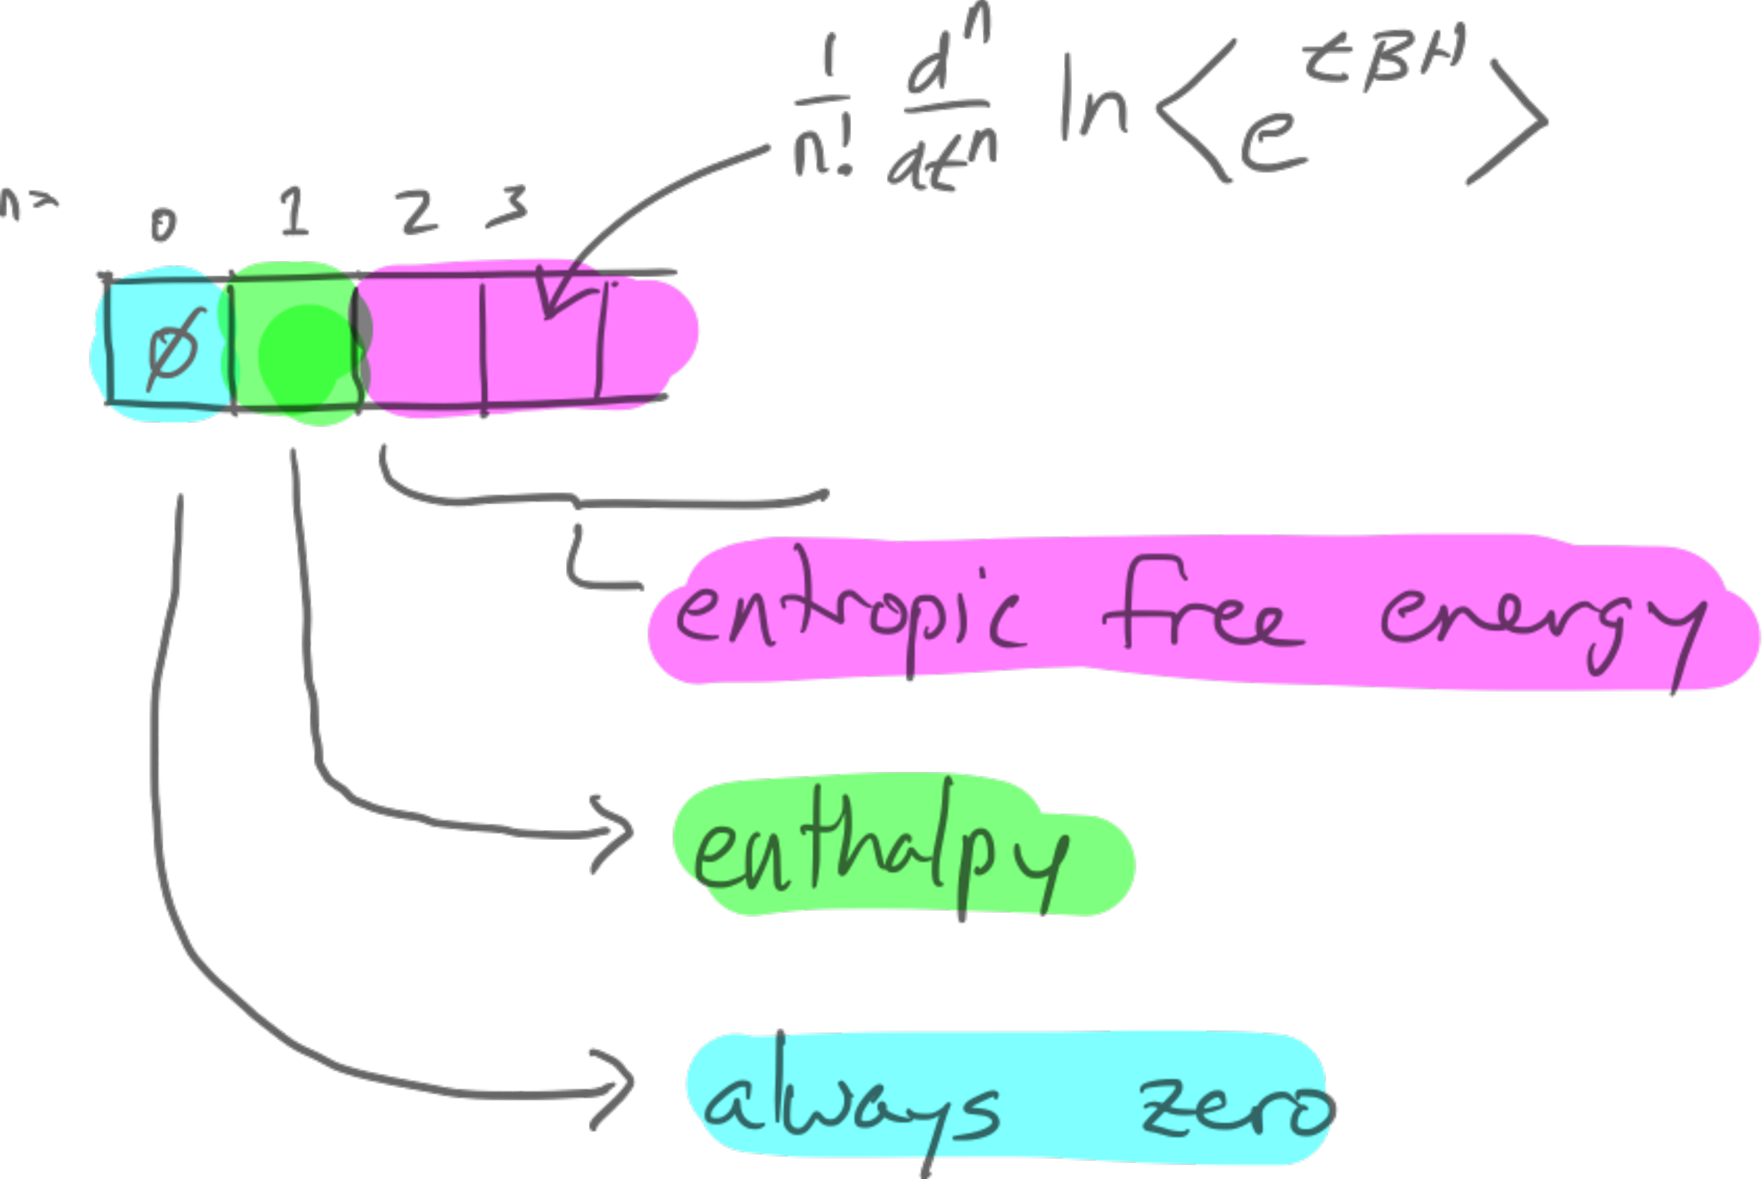
\includegraphics[width=3in]{figure1.pdf}
\caption{Graphical breakdown of the free energy in terms of cumulants.}
\label{fig:1D}
\end{figure}

We can recast Eq.~\ref{eq:cumu_dA} graphically as a sum over an infinite 1-dimensional array of cells (Figure~\ref{fig:1D}), where the $n$th cell contains the $n$th cumulant along with the factor $\beta^{-1}/n!$. The first cell ($n=0$) is always zero. The next cell ($n=1$) is the enthalpy, $\langle H \rangle_\lambda$. The sum of the remaining cells ($n=2...$) is the entropic free energy.

This breakdown makes sense, as the enthalpy is simply the average energy of the system, which is exactly the first cumulant. Meanwhile, the entropic part of the free energy depends on the ``peakedness'' or ``flatness'' of the ensemble, which is exactly what is characterized by the the higher-order cumulants.

% Several properties of cumulants have important statistical mechanical implications. First, the cumulants are semi-invariant, meaning that $\kappa_1(X+c)=\kappa_1(X)+c$ and $\kappa_n(X+c) = \kappa_n(X)$ for some constant $c$ and $n \ge 2$. In statistical mechanics, this implies that if the energy of every microstate in a system is changed by $c$, the enthalpy also increases by $c$, whereas the entropy is unchanged. Second, the cumulants are additive $\kappa_n(X + Y) = \kappa_n(X) + \kappa_n(Y)$ when $X$ and $Y$ are independent. In statistical mechanics, this implies that for a composite system composed of independent sub-systems, the the total enthalpy or entropy is just the sum of the sub-system enthalpies or entropies.

\subsection{The free energy can be decomposed using a multivariate cumulant expansion.}

We can also relate Eq.~\ref{eq:avg_expr} to the multivariate cumulant generating function for the random variables $\beta H_1$ and $\beta H_2$, defined as:
\begin{equation}
K_\lambda(\vec t) =
	\ln \left\langle 
    	e^{t_1 \beta H_1(\lambda) + t_2 \beta H_2(\lambda)}
    \right\rangle_\lambda.
\end{equation}
Series expansion around $\vec t = (t_1, t_2) = 0$ gives:
\begin{align}
\Delta A(\lambda) =& \beta^{-1} K_\lambda(1, 1) \nonumber\\
                  =& \beta^{-1} \sum_{n=1}^{\infty}
	        			\sum_{i+j=n}
            			\frac{1}{i!j!}\left[ D_{i,j} K_\lambda\right]_{\vec t=0},
\label{eq:mult_expansion}
\end{align}
where the notation $D_{i,j}$ means $d^{i+j} /(d t_1^i d t_2^j)$ and the second sum is over non-negative $i$ and $j$. This expansion readily generalizes to an arbitrary number of Hamiltonian components. 

The mixed derivatives with both $i>0$ and $j>0$ give the joint cumulants, which characterize the statistical dependence of $H_1$ and $H_2$ to a given order $n=i+j$. See Appendix 1 for a discussion of their intuitive meaning.




\subsection{The free energy can be decomposed into univariate and multivariate terms.}

\begin{figure}[tb]
\centering
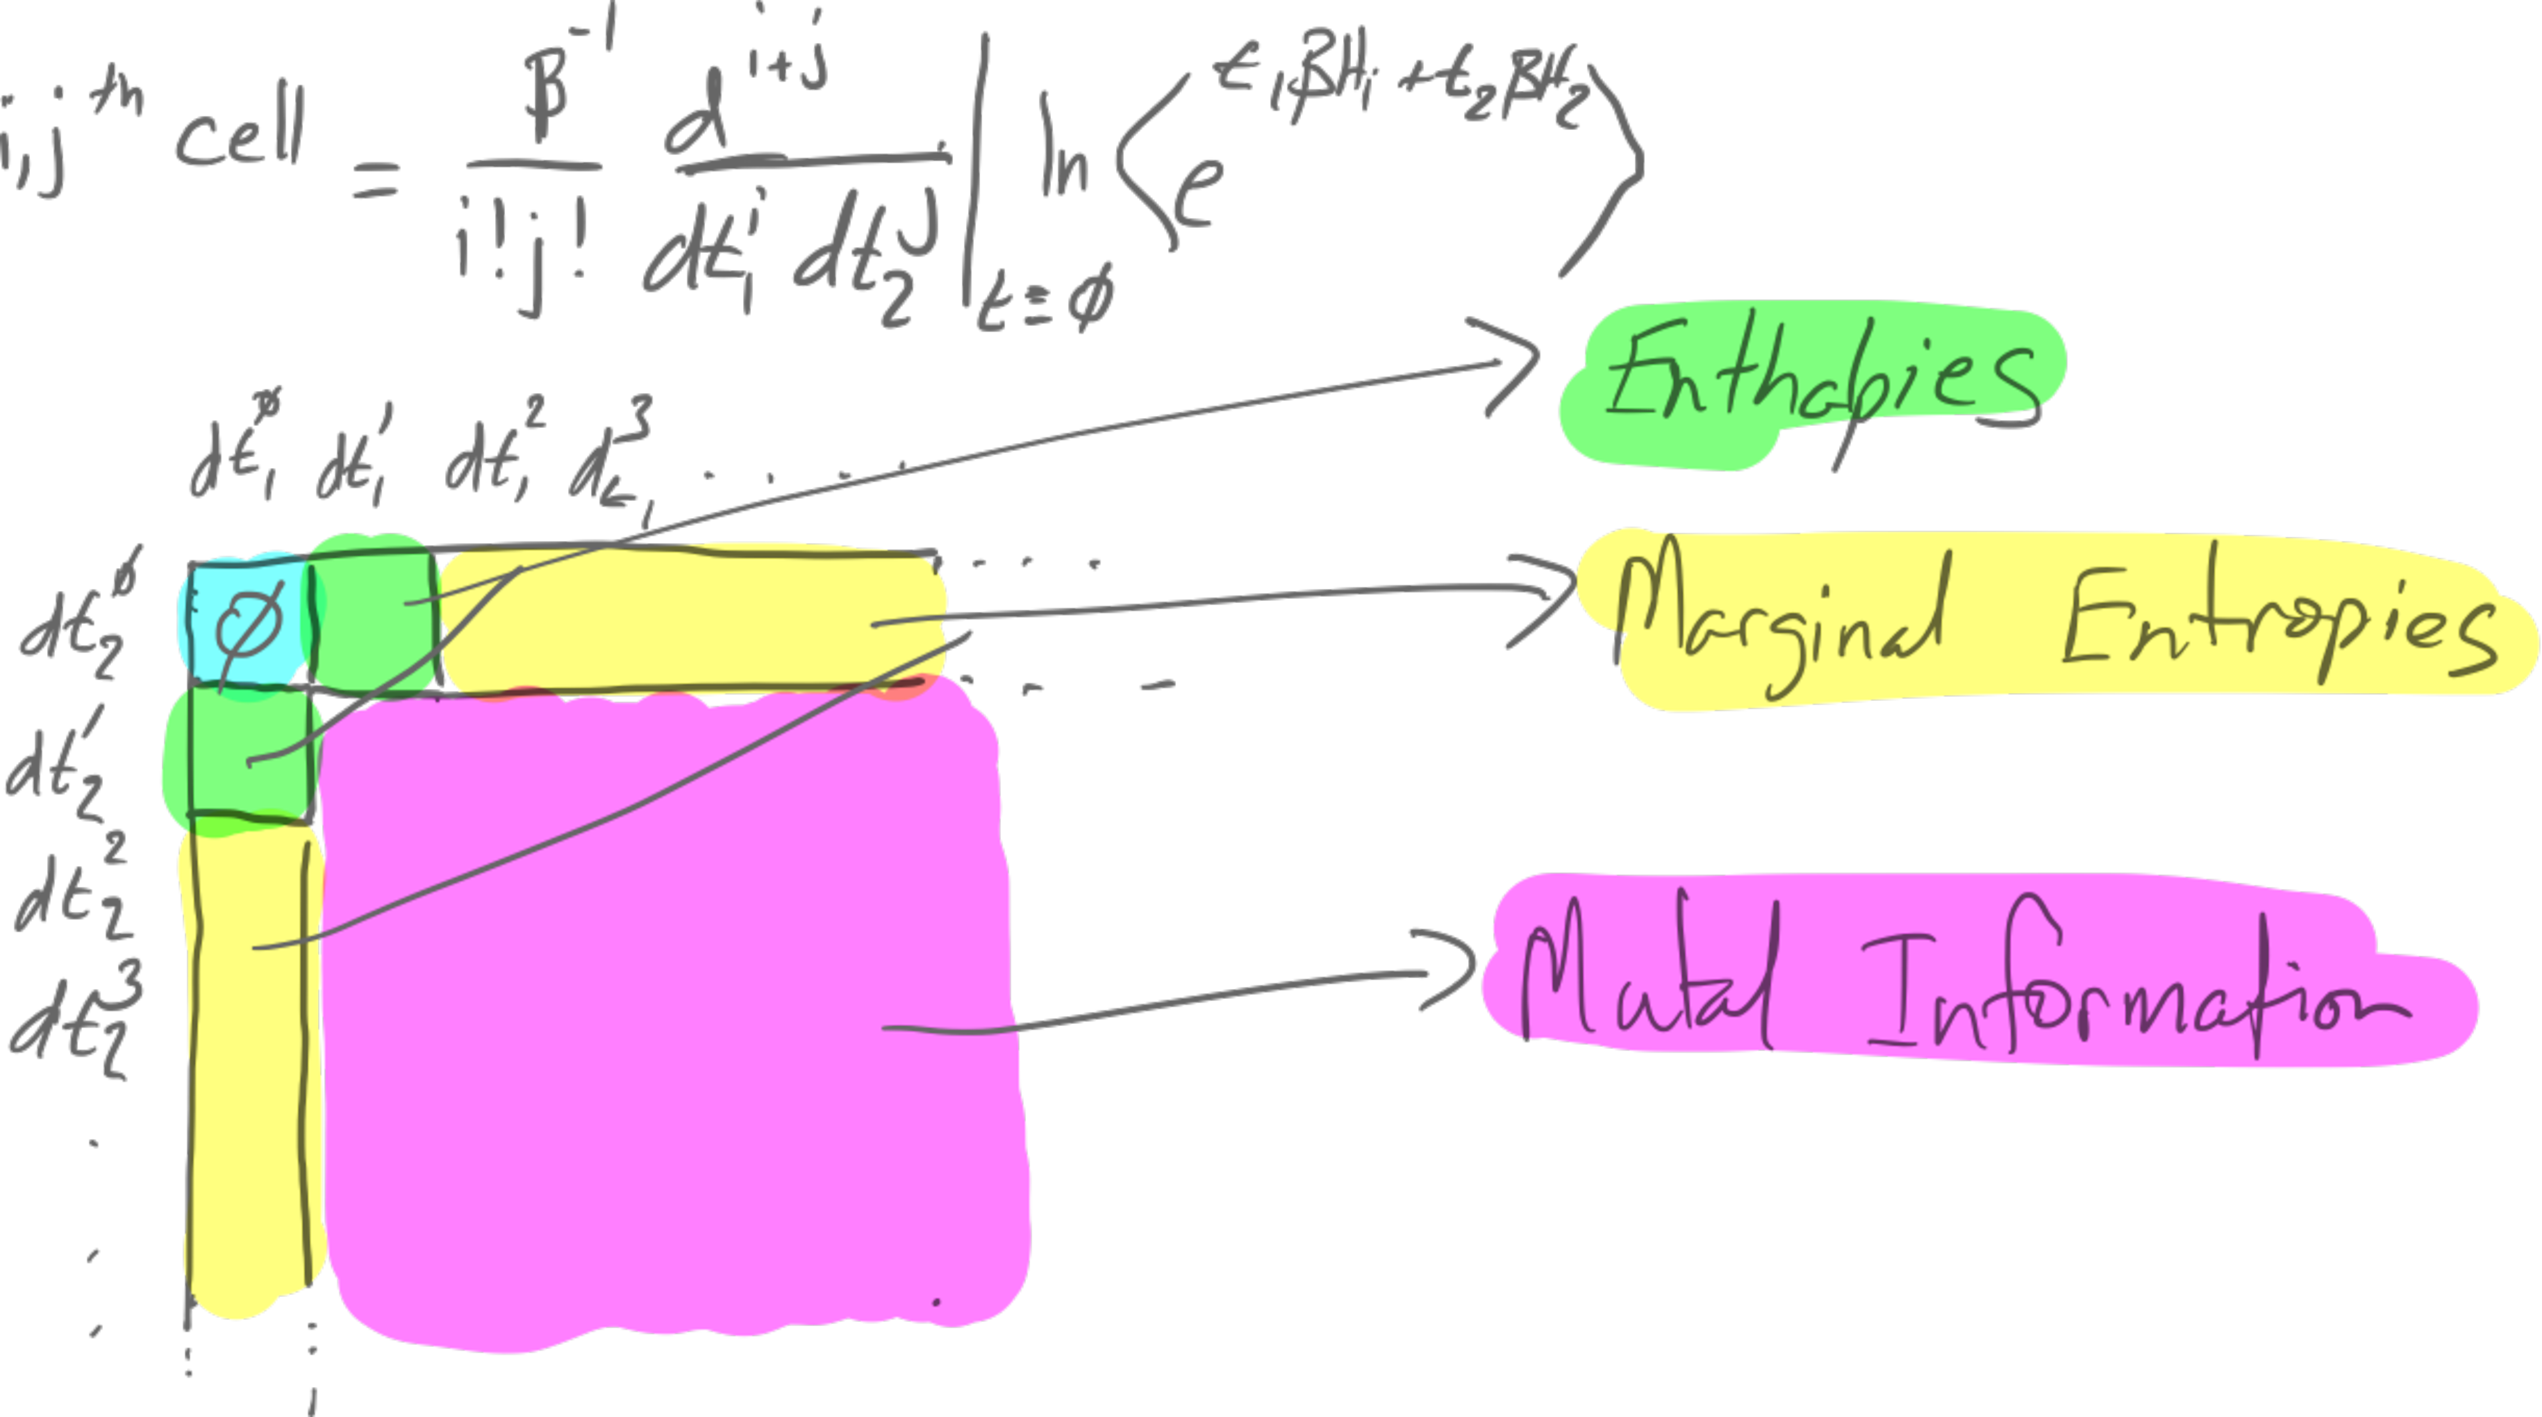
\includegraphics[width=3in]{figure2.pdf}
\caption{Graphical breakdown of free energy in terms of multivariate cumulants.}
\label{fig:2D}
\end{figure}

Eq.~\ref{eq:mult_expansion} can be also be recast graphically, but this time as the sum of an infinite 2-dimensional array (Figure~\ref{fig:2D}). The $i,j=(0,0)$ cell is always zero. The $(1,0)$ and $(0,1)$ cells are the enthalpic components $\langle H_1 \rangle_\lambda$ and $\langle H_2 \rangle_\lambda$, respectively. The sum of the remaining terms is the entropic free energy. 

We note that the cumulant of order $n$ in the univariate expansion is the sum of the cumulants where $i+j=n$ in the multivariate expansion, as shown in Figure~\ref{fig:cumsum}.

\begin{figure}[htb]
\centering
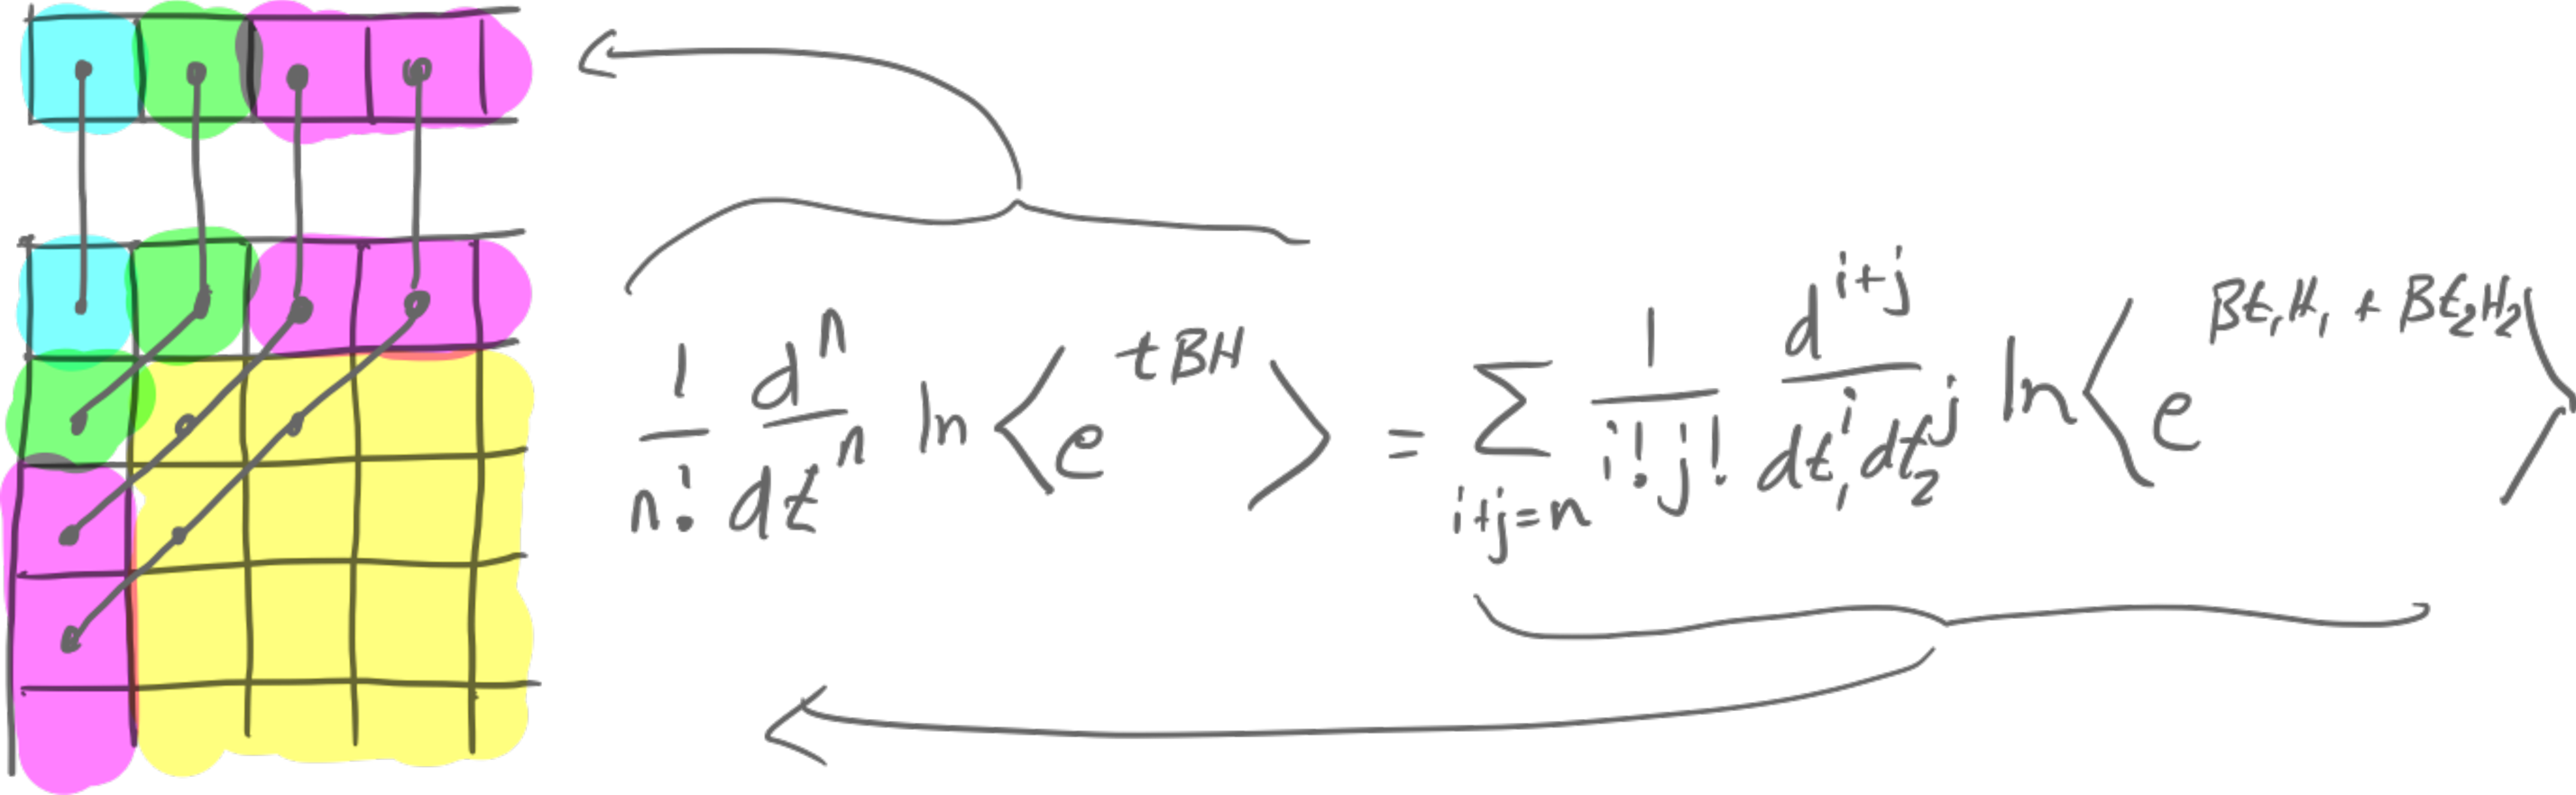
\includegraphics[width=3in]{figure3.pdf}
\caption{The multivariate cumulants to a given order sum to the univariate cumulant of the same order.}
\label{fig:cumsum}
\end{figure}


The entropic free energy can further be decomposed (Figure~\ref{fig:2D}) into two univariate marginal entropic contributions, $\mathcal{S}(H_1)$ and $\mathcal{S}(H_2)$, magenta region, and a bivariate joint entropic contribution, $\mathcal{S}(H_1, H_2)$, yellow region.

This graphical decomposition extends to higher dimensions, although it becomes difficult to visualize. As shown in Figure X, a three component Hamiltonian would have:
\begin{itemize}
	\item three enthalpies: $\langle H_1 \rangle_\lambda$, $\langle H_2 \rangle_\lambda$, $\langle H_3 \rangle_\lambda$,
	\item three univariate entropic contributions: $\mathcal{S}(H_1)$, $\mathcal{S}(H_2)$, $\mathcal{S}(H_3)$,
	\item three bivariate entropic contributions: $\mathcal{S}(H_1, H_2)$, $\mathcal{S}(H_1, H_3)$, $\mathcal{S}(H_2, H_3)$, 
	\item and a single trivariate entropic contribution: $\mathcal{S}(H_1, H_2, H_3)$.
\end{itemize}

Note that we use the notation $\mathcal{S}(H_i)$ to indicate the entropic free energy contribution to the free energy due to $H_i$, rather than the entropy of the random variable $H_i$ itself. Multivariate contributions, like $\mathcal{S}(H_1, H_2)$, include only the cumulant terms where all of the corresponding derivative terms are non-zero. In other words, the $\mathcal{S}(H_1)$ and $\mathcal{S}(H_2)$ terms are not included in $\mathcal{S}(H_1, H_2)$.






\subsection{Splitting the cumulants results in a path-independent free energy decomposition.}

The cumulants are state functions, so we can define path-independent free energy decompositions by splitting the cumulants between the different components:
\begin{equation}
\Delta A^{(u)}(\lambda) =
	\beta^{-1} \sum_{n=1}^{\infty}
	\sum_{i+j=n}
	\frac{a_{i,j}^{(u)}}{i!j!}\left[ D_{i,j} K_\lambda\right]_{t=0},
\end{equation}
where $u=1, 2, \ldots$ indexes the components, and $a_{i,j}^{(u)}$ are the splitting coefficients. The splitting coefficients divide each cumulant between the free energy components and are subject to $0 \le a_{i,j}^{(u)} \le 1$ and $\sum_u a_{i,j}^{(u)}=1$.

The free energy components can be evaluated by thermodynamic integration:
\begin{align}
\Delta\Delta A^{(u)} =& \Delta A^{(u)}(1) - \Delta A^{(u)}(0) \nonumber \\
					 =&
	\beta^{-1} \int_0^1 \sum_{n=1}^{\infty}
	\sum_{i+j=n}
	\frac{a_{i,j}^{(u)}}{i!j!}
    \left[ D_{i,j} \frac{dK_\lambda}{d\lambda}\right]_{t=0} d\lambda
    \label{eq:split}.
\end{align}
Only in a few cases do most of terms in Eq.~\ref{eq:split} cancel. In the general case, an infinite number of terms are present. However, we show below that we are able to partially correct a path-dependent free energy decomposition by correctly splitting the low order cumulants, while leaving a path-dependent splitting of the higher-order terms. We will further show that, in some cases, the infinite sum can be reorganized into a Taylor series that can be recognized as an ensemble average.

Evaluating the derivative of the cumulant generating function with respect to $\lambda$ gives:
\begin{equation}
K_\lambda' = 
\frac{dK_\lambda}{d\lambda} =
	\beta \left[
		t_1 \left\langle H_1' \right\rangle_{\vec t,\lambda} -
    	\left\langle H_1' \right\rangle_{\vec t,\lambda} +
	    t_2 \left\langle H_2' \right\rangle_{\vec t,\lambda} -
    	\left\langle H_2' \right\rangle_{\vec t,\lambda}
    \right]
\end{equation}
where we have dropped terms with no $\vec t$-dependence that will disappear in subsequent steps, the prime indicates the derivative with respect to $\lambda$, and the notation $\langle X \rangle_{\vec t, \lambda}$ means
\begin{equation}
\langle X \rangle_{\vec t, \lambda}  =
	\frac
    	{\int X(x, \lambda) 
        	\exp\left[
        		\beta(t_1-1)H_1(\lambda) +
            \beta(t_2-1)H_2(\lambda)
        \right] dx
        }
    	{\int
        	\exp\left[
            \beta(t_1-1)H_1(\lambda) +
            \beta(t_2-1)H_2(\lambda)
        \right] dx
        }.
\end{equation}

The general form of $D_{i,j}K'$ is:
\begin{equation}
[D_{i,j}K_\lambda']_{\vec t=0} =
	\beta\left[
		i \phi_{i-1, j}^{(1)}(\lambda) -
    	\phi_{i,j}^{(1)}(\lambda) +
    	j \phi_{i, j-1}^{(2)}(\lambda) -
    	\phi_{i,j}^{(2)}(\lambda)
    \right],
\label{eq:deriv}
\end{equation}
where we have introduced the notation
\begin{equation}
\phi_{i,j}^{(u)}(\lambda) =
	\left[ D_{i,j} \left\langle
    	H_u'
    \right\rangle_{\vec t, \lambda} \right]_{\vec t=0}.
\end{equation}
Each term $\phi_{i,j}^{(1)}$ can be produced in two different ways, from $D_{i,j}K'$ or $D_{i+1,j}K'$. Similarly, each $\phi_{i,j}^{(2)}$ can be produced from $D_{i,j}K'$ or $D_{i,j+1}K'$.

Regrouping similar terms, we can rewrite Eq.~\ref{eq:split} as:
\begin{equation}
\Delta\Delta A^{(u)} =
	\int_0^1 \left(
        a_{1,0}^{(u)}\left\langle H_1' \right\rangle +
        a_{0,1}^{(u)}\left\langle H_2' \right\rangle +
        \psi_1^{(u)}(\lambda) +
        \psi_2^{(u)}(\lambda)
    \right) d\lambda,
\label{eq:dA_expansion}
\end{equation}
with
\begin{align}
\psi_1^{(u)}(\lambda) &=
%	\sum_{n=1}^{\infty}
%    \sum_{i+j=n}
%        \phi_{i,j}^{(1)}\left(
%            \frac
%                {(i+1)a_{i+1,j}^{(u)}}
%                {(i+1)!j!} -
%            \frac
%                {a_{i,j}^{(u)}}
%                {i!j!}
%        \right) \nonumber\\
%    &=
	\sum_{n=1}^{\infty}
    \sum_{i+j=n}
        \frac{\phi_{i,j}^{(1)}}{i!j!}
        \left(
            {a_{i+1,j}^{(u)}} -
            {a_{i,j}^{(u)}}
        \right) \label{eq:psi1}\\
\psi_2^{(u)}(\lambda) &=
	\sum_{n=1}^{\infty}
    \sum_{i+j=n}
        \frac{\phi_{i,j}^{(2)}}{i!j!}
        \left(
            a_{i,j+1}^{(u)} -
            a_{i,j}^{(u)}
      	\right)\label{eq:psi2}.
\end{align}



\subsection{Most terms cancel in the expression for the total free energy.}

Consider the case where there is only a single free energy component, i.e. the total free energy. In this case, the splitting coefficient is always unity, $a_{i,j}^\mathrm{total}=1$. Under these conditions, the bracketed terms in Eqs.~\ref{eq:psi1} and \ref{eq:psi2} evaluate to zero and the free energy is:
\begin{equation}
\Delta\Delta A = \int_0^1 \bigg(
	\left\langle H_1' \right\rangle +
    \left\langle H_2' \right\rangle
\bigg) d\lambda,
\end{equation}
which is equivalent to Eq.~\ref{eq:TI} as expected.





\subsection{There are no non-trivial splittings for arbitrary $\lambda$-dependence.}

Consider an arbitrary $\lambda$-dependence of the Hamiltonian. Cancellation of the bracketed terms in Eqs.~\ref{eq:psi1} and \ref{eq:psi2} requires that
\begin{align*}
a_{i+1,j}^{(u)} &= a_{i,j}^{(u)} \\
a_{i,j+1}^{(u)} &= a_{i,j}^{(u)},
\end{align*}
which has only trivial solutions like $a_{i,j}^{(1)} = a_{i,j}^{(2)} = 1/2$ that partition the free energy into fixed fractions of the total.

In Appendix 2, we show that the particular case of an identical scaling, $H(\lambda) = f(\lambda)h_1 + f(\lambda)h_2$ for some arbitrary real function $f(\lambda)$, results in a well-defined splitting of the cumulants with nearly complete cancelation of terms, in agreement with previous results. However, this functional form is quite limiting and not appropriate for many systems, and while the splitting produced under these conditions is path-independent, it does not have a particularly obvious interpretation.








\subsection{Good decompositions are readily interpretable and make predictions.}

Provided the splitting coefficients are valid, that is $0 \le a_{i,j}^{(u)} \le 1$ and $\sum_u a_{i,j}^{(u)}=1$, no decomposition is more correct than any other. However, some decompositions are not useful, as they are difficult to interpret and provide little or no predictive power (Figure~\ref{fig:bad_split}).

\begin{figure}[tb]
\centering
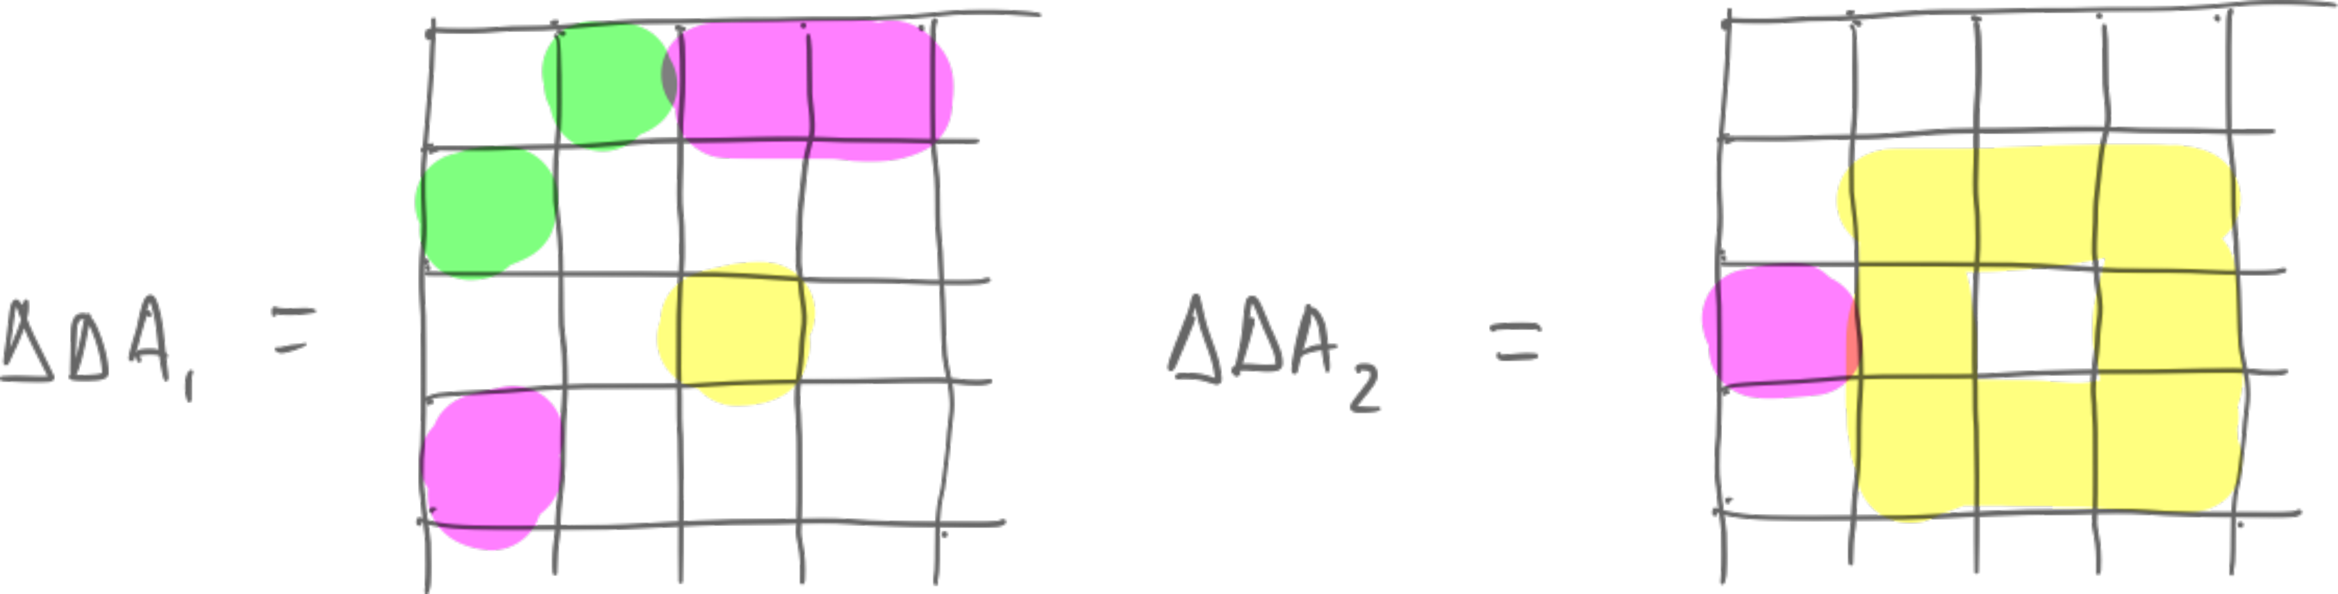
\includegraphics[width=3in]{figure6.pdf}
\caption{An example of a decomposition that is difficult to interpret and makes no useful predictions.}
\label{fig:bad_split}
\end{figure}

\begin{figure}[tb]
\centering
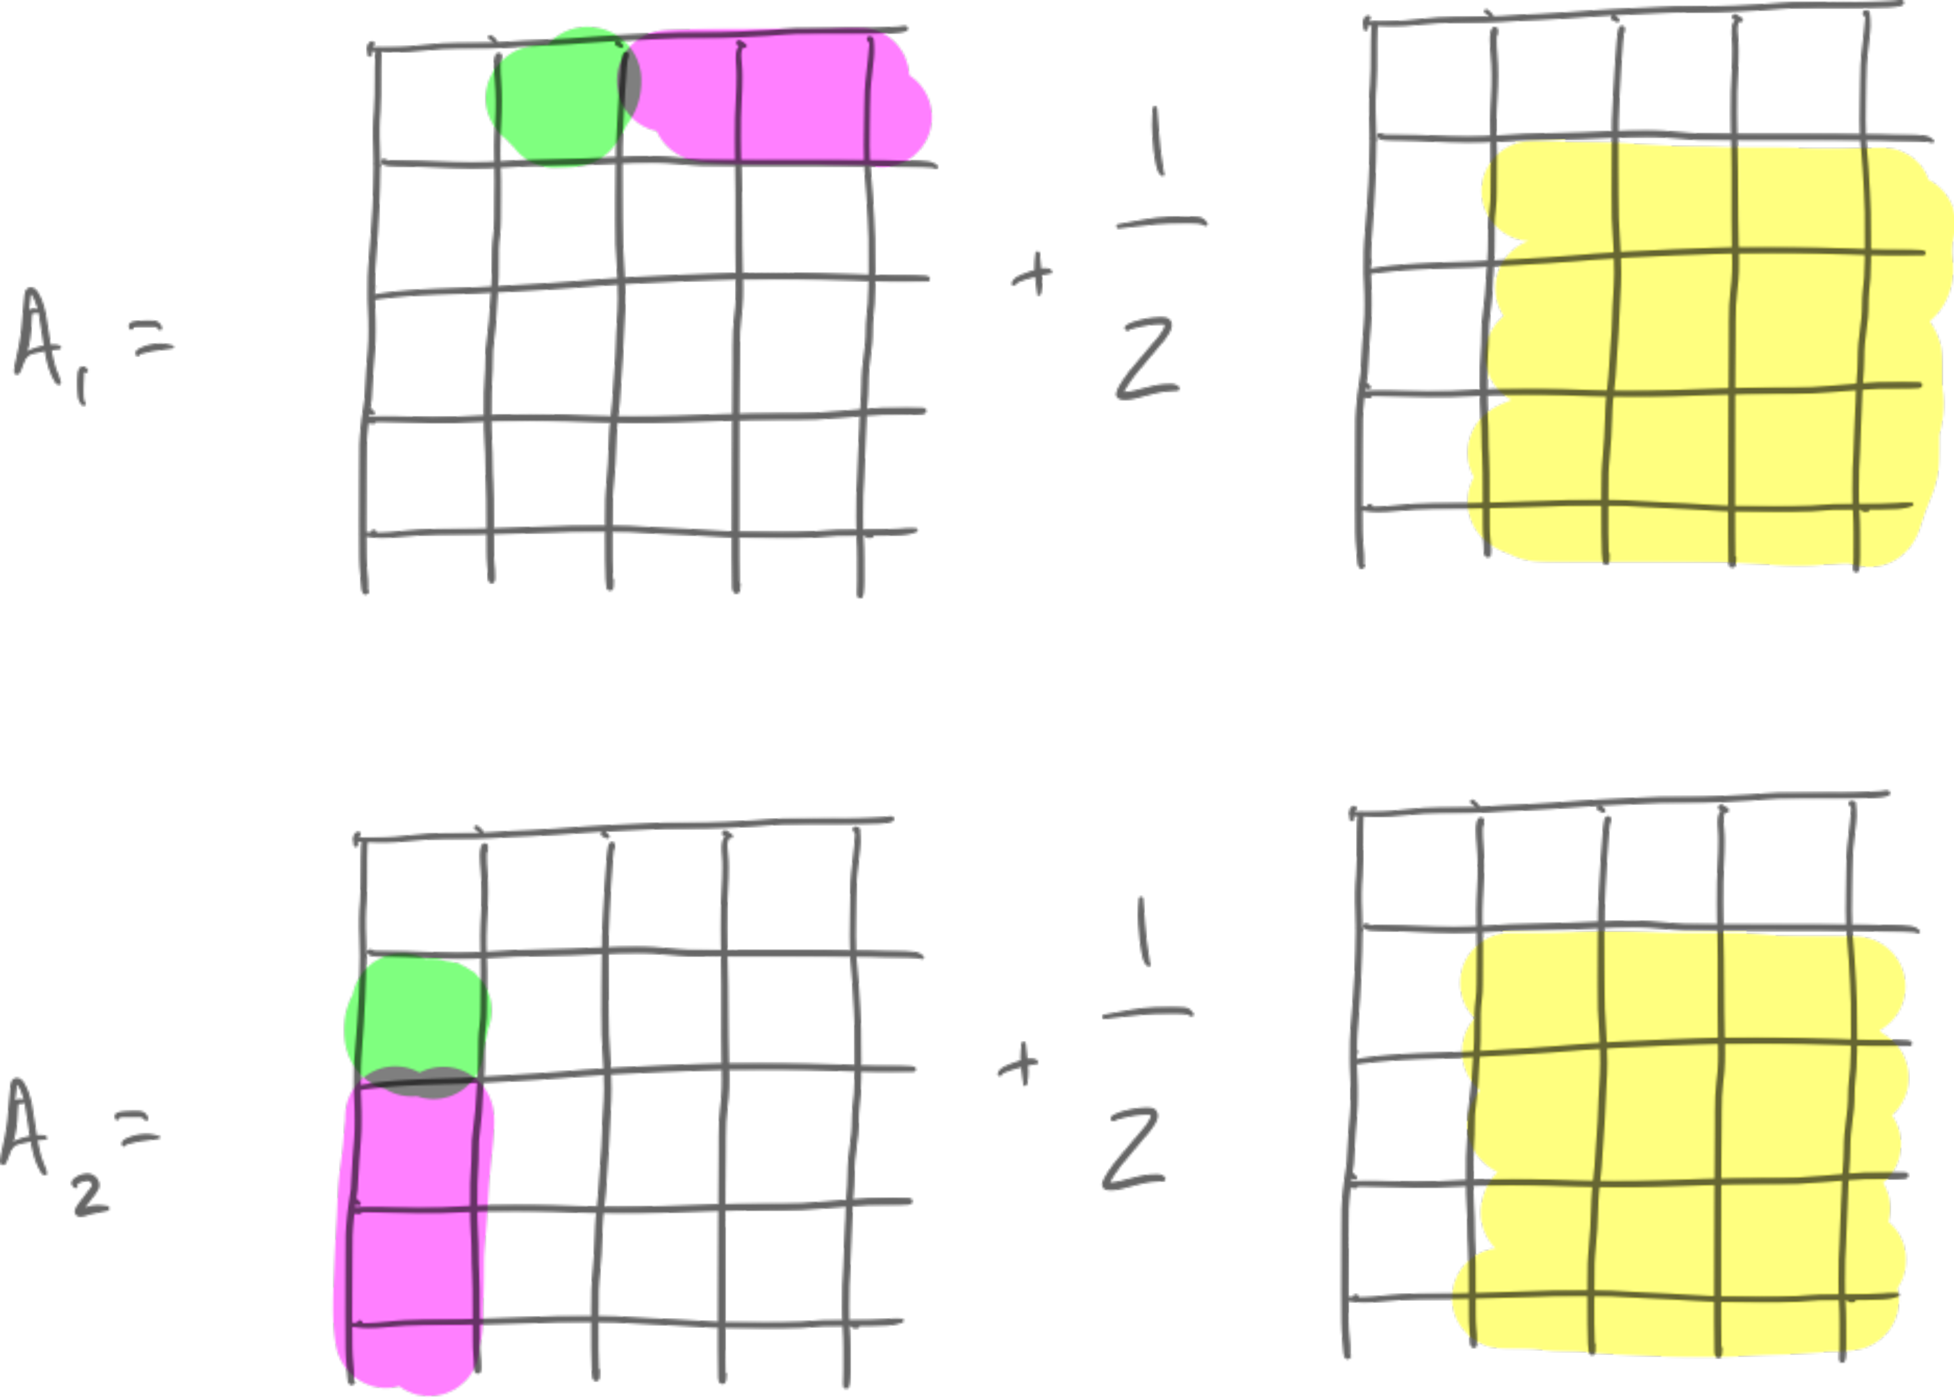
\includegraphics[width=3in]{figure4.pdf}
\caption{An example of a decomposition that is easy to interpret, but where predictions are difficult to make.}
\label{fig:ok_split}
\end{figure}

Some decompositions are more readily interpretable, e.g. Figure~\ref{fig:ok_split}. This splitting decomposes the cumulants in a obvious way, with half of each joint cumulant split between the two components. However, this decompositions does not allow us to make predictions. For example, what would the free energy be if $H_1$ was set to zero? This decomposition does not allow us to address this question.


Figure~\ref{fig:good_split} shows an example of the most useful type of decomposition. In this decomposition, $\Delta\Delta A_1$ contains all of the cumulants to depend only on $H_1$, $\Delta\Delta A_2$ contains all of the cumulants that depend only on $H_2$, and $\Delta\Delta A_{12}$ contains all of the cumulants that depend on both $H_1$ and $H_2$. This decomposition is readily interpretable, as each component has a clear meaning. Furthermore, this decompositions enables predictions due to an important property of cumulants: any component that contains one or more variables that is independent of all others vanishes. So for example, if $H_1$ is set to zero, then $\Delta\Delta A_1$ and $\Delta\Delta A_{12}$ vanish, leaving only $\Delta\Delta A_2$.

\begin{figure}[tb]
\centering
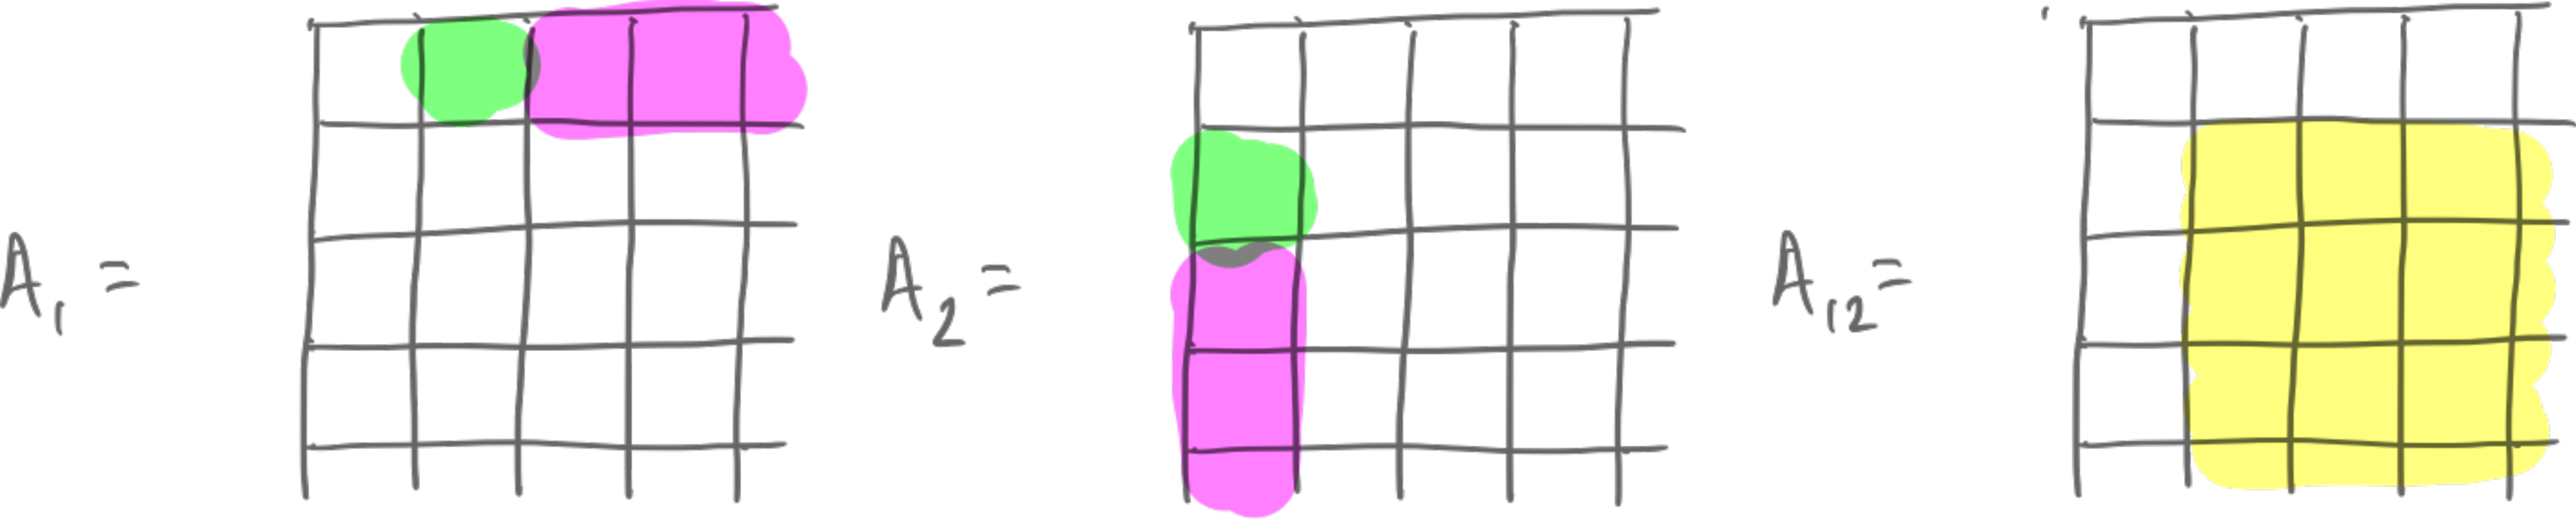
\includegraphics[width=3in]{figure5.pdf}
\caption{It is advantageous to partition joint entropic contributions into their own free energy components.}
\label{fig:good_split}
\end{figure}




\subsection{The path-dependence of free energy decompositions can be partially eliminated by performing a correction to finite order.}

Consider the sum of terms due to $\psi_1$:
\begin{align*}
\sum_u \psi_1^{(u)} =&
	\sum_{n=1}^{\infty}
    \sum_{i+j=n}
        \frac{\phi_{i,j}^{(1)}}{i!j!}
        \left(
        		\sum_u a_{i+1,j}^{(u)} -
        		\sum_u a_{i,j}^{(u)}
        \right) = 0,
\end{align*}
where the second equality holds because each set of splitting coefficients sums to unity. A similar result holds for the terms due to $\psi_2$.

We can view each order $n$ of Eqs.~\ref{eq:psi1} and \ref{eq:psi2} as a correction towards a particular path-independent splitting. Each order of correction leaves the total free energy invariant, but shifts some free energy between the components. Thus, the path-dependence can be partially corrected by truncating Eqs.~\ref{eq:psi1} and \ref{eq:psi2} at finite order without affecting the total free energy.








\subsection{Some decompositions lead to infinite series that can be identified as Taylor series.}

Consider the decomposition given in Figure~\ref{fig:good_split}:
\begin{align*}
a_{i,j}^{(1)} =&
	\begin{cases}
	1 &\text{if}\ i>0,  j=0 \\
	0 &\text{otherwise}
	\end{cases} \\
a_{i,j}^{(2)} =&
	\begin{cases}
	1 &\text{if}\ i=0,  j>0 \\
	0 &\text{otherwise}
	\end{cases} \\
a_{i,j}^{(12)} =&
	\begin{cases}
	1 &\text{if}\ i>0,  j>0 \\
	0 &\text{otherwise}.
	\end{cases}
\end{align*}
Substituting $a_{i,j}^{(1)}$ into Eq.~\ref{eq:dA_expansion} gives:
\begin{align}
\frac{dA_1}{d\lambda} =& 
	\left\langle
		\frac{dH_1}{d\lambda}
	\right\rangle_\lambda -
	\phi_{1,0}^{(2)} -
	\frac{1}{2} \phi_{2,0}^{(2)} -
	\frac{1}{6} \phi_{3,0}^{(2)} - \ldots \nonumber\\
	=&
	\left\langle
		\frac{dH_1}{d\lambda}
	\right\rangle_\lambda -
	\sum_{n=1}^{\infty} \frac{1}{n!} \phi_{n,0}^{(2)}.
\label{eq:almost_taylor}
\end{align}
If we define $f(t)$ as:
\begin{equation}
f(t) = \frac
	{\int H_2' e^{\beta(t-1) H_1 - \beta H_2} dx}
	{\int e^{\beta(t-1) H_1 - \beta H_2} dx},
\end{equation}
we see that the sum in Eq.~\ref{eq:almost_taylor} is almost the series expansion of $f(1)$. Adding and subtracting the missing zeroth order term gives:
\begin{align}
\frac{dA_1}{d\lambda} =&
	\left\langle
		\frac{dH_1}{d\lambda}
	\right\rangle_\lambda +
	f(0) -
	\left(
		\sum_{n=1}^{\infty} \frac{1}{n!}
		\left[ \frac{d^n}{dt^n} f(t) \right]_{t=0}
		+ f(0)
	\right)\nonumber\\
=&
	\left\langle
		\frac{dH_1}{d\lambda}
	\right\rangle_\lambda +
	\left\langle
		\frac{dH_2}{d\lambda}
	\right\rangle_\lambda -
	\frac
		{\int H_2' e^{-\beta H_2} dx}
		{\int e^{-\beta H_2} dx} \nonumber\\
=&
	\left\langle
		\frac{dH_1}{d\lambda}
	\right\rangle_\lambda +
	\left\langle
		\frac{dH_2}{d\lambda}
	\right\rangle_\lambda -
	\left\langle
		H_2'
	\right\rangle_{\lambda, H_1=0} \label{eq:diff_ensemble}\\
=&
	\left\langle
		\frac{dH_1}{d\lambda}
	\right\rangle_\lambda +
	\left\langle
		\frac{dH_2}{d\lambda}
	\right\rangle_\lambda -
	\frac
		{\left\langle H_2' e^{\beta H_1} \right\rangle_\lambda}
		{\left\langle e^{\beta H_1} \right\rangle_\lambda}
	\label{eq:same_ensemble}
\end{align}
This says that free energy component $\Delta A_1$ is equal to the total free energy less the free energy that would be obtained if $H_1$ were zero.

Eq.~\ref{eq:diff_ensemble} expresses this as an average over an ensemble where $H_1$ is zero, whereas Eq.~\ref{eq:same_ensemble} expresses this as an average over the regular ensemble with an additional weighting factor of $e^{\beta H_1}$.

The relationship between Eq.~\ref{eq:same_ensemble} and Eq.~\ref{eq:almost_taylor} is similar to that encountered when using cumulant expansions to estimate free energy changes from non-equilibrium simulations using the Jarzynski inequality. Truncating Eq.~\ref{eq:almost_taylor} at a finite order introduces error. However, the exponential in Eq.~\ref{eq:same_ensemble} can be very noisy, so depending on the system and on sampling, one form or the other may be more accurate.

Applying the same analysis to all three components gives:
\begin{align*}
\frac{dA_1}{d\lambda} =&
	\left\langle
		H_1'
	\right\rangle_\lambda +
	\left\langle
		H_2'
	\right\rangle_\lambda -
	\frac
		{\left\langle H_2' e^{\beta H_1} \right\rangle_\lambda}
		{\left\langle e^{\beta H_1} \right\rangle_\lambda} \\
\frac{dA_2}{d\lambda} =&
	\left\langle
		H_1'
	\right\rangle_\lambda +
	\left\langle
		H_2'
	\right\rangle_\lambda -
	\frac
		{\left\langle H_1' e^{\beta H_2} \right\rangle_\lambda}
		{\left\langle e^{\beta H_2} \right\rangle_\lambda} \\
\frac{dA_{1,2}}{d\lambda} =&
	\frac
		{\left\langle H_2' e^{\beta H_1} \right\rangle_\lambda}
		{\left\langle e^{\beta H_1} \right\rangle_\lambda} +
	\frac
		{\left\langle H_1' e^{\beta H_2} \right\rangle_\lambda}
		{\left\langle e^{\beta H_2} \right\rangle_\lambda} -
	\left\langle
		H_1'
	\right\rangle_\lambda -
	\left\langle
		H_2'
	\right\rangle_\lambda
\end{align*}





\section{Numerical Results}

\section{Conclusions}

\section*{Appendices}
\subsection*{Appendix 1. The joint cumulants capture the statistical dependence of Hamiltonian components.}

The mixed partial derivatives with respect to $\vec t$ capture the statistical dependence of Hamiltonian components to a given order. For example, the second order $\kappa_{0,1,1}$ term is simply the covariance between $H_1$ and $H_2$:
\begin{align}
\kappa_{0, 1, 1} = [D_{0, 1, 1} K_\lambda]_{\vec t=0} =&
	\beta^2 \left[
    	\left\langle H_1 H_2 \right\rangle_\lambda -
		\left\langle H_1 \right\rangle_\lambda 
		\left\langle H_2 \right\rangle_\lambda
    \right] \nonumber\\
    =&
    \beta^2 \mathrm{Cov}(H_1,H_2).              
\end{align}
This cumulant the difference between the actual average value of the product of $H_1$ and $H_2$ compared to that expected if $H_1$ and $H_2$ were statistically independent.

Similarly, the third order cumulant, $\kappa_{1,1,1}$, captures the difference between the average product of $H_0$, $H_1$, and $H_2$ compared to what is expected if they were statistically independent:
\begin{alignat}{3}
\MoveEqLeft[3] [D_{1, 1, 1} K_\lambda]_{\vec t=0}\notag\\
&= \beta^3[ &&
\left\langle H_0 H_1 H_2 \right\rangle_\lambda -
\left\langle H_0 H_1 \right\rangle_\lambda
	\left\langle H_2 \right\rangle_\lambda -
\left\langle H_0 H_2 \right\rangle_\lambda
	\left\langle H_1 \right\rangle_\lambda - \notag\\
&&& \left\langle H_1 H_2 \right\rangle_\lambda
	\left\langle H_0 \right\rangle_\lambda +
2 \left\langle H_0 \right\rangle_\lambda
	\left\langle H_1 \right\rangle_\lambda
	\left\langle H_2 \right\rangle_\lambda]\notag\\
&= \beta^3[ &&
	\left\langle H_0 H_1 H_2 \right\rangle_\lambda -
	\mathrm{Cov}(H_0,H_1) \left\langle H_2 \right\rangle_\lambda -
	\mathrm{Cov}(H_0,H_2) \left\langle H_1 \right\rangle_\lambda -\\
	&&& \mathrm{Cov}(H_1,H_2) \left\langle H_0 \right\rangle_\lambda -
	\left\langle H_0 \right\rangle_\lambda
		\left\langle H_1 \right\rangle_\lambda
		\left\langle H_2 \right\rangle_\lambda]        
\end{alignat}
This cumulant accounts for all of the ways that there can be independence, where either all three variables being independent, or where two of the variables are dependent, but the third is independent.

Expressions for higher-order cumulants rapidly become more complex, but they all capture the same...





\subsection{Appendix 2. Identical scaling leads to a natural splitting where most terms cancel.}

Consider the case where the $\lambda$-dependence is an identical scaling, $H(\lambda) = f(\lambda)h_1 + f(\lambda)h_2$. In these circumstances,
\begin{equation*}
\frac{\partial}{\partial t_1}
	\langle H_2' \rangle_{\vec t, \lambda} = 
\frac{\partial}{\partial t_2}
	\langle H_1' \rangle_{\vec t, \lambda},
\end{equation*}
which implies
\begin{equation}
\phi_{i,j}^{(2)} = \phi_{i-1,j+1}^{(1)}.
\label{eq:separable}
\end{equation}
Substitution of Eq.~\ref{eq:separable} into Eq.~\ref{eq:deriv} gives
\begin{align}
[D_{i,j}K_\lambda']_{\vec t=0} &=
	\beta\left[
		i \phi_{i-1, j}^{(1)}(\lambda) -
    	\phi_{i,j}^{(1)}(\lambda) +
    	j \phi_{i-1, j}^{(1)}(\lambda) -
    	\phi_{i-1,j+1}^{(1)}(\lambda)
    \right] \nonumber \\
    &=
	\beta\left[
		(i + j)\phi_{i-1, j}^{(1)}(\lambda) -
    	\phi_{i,j}^{(1)}(\lambda) -
    	\phi_{i-1,j+1}^{(1)}(\lambda)
    \right].
\end{align}
Each term $\phi_{i,j}^{(1)}$ can be produced in three different ways, from $D_{i,j}K'$, $D_{i+1,j}K'$, or $D_{i+1,j-1}K'$. Grouping of similar terms gives
\begin{equation}
\Delta\Delta A^{(u)} =
	\int_0^1 \left(
        a_{1,0}^{(u)}f'(\lambda)
        \left\langle h_1 \right\rangle +
        a_{0,1}^{(u)}f'(\lambda)
        \left\langle h_2 \right\rangle +
        \sigma(\lambda)
    \right) d\lambda,
\end{equation}
with
\begin{align}
\sigma(\lambda) &=
	\sum_{n=1}^{\infty}
    \sum_{i+j=n}
        \frac
        	{\phi_{i,j}^{(1)}}
            {i!j!}
        \left(
            \frac
                {(i+j+1)a_{i+1,j}^{(u)}}
                {i+1} -
            a_{i,j}^{(u)} -
           	\frac
            	{j a_{i+1,j-1}^{(u)}}
                {i+1}
		\right).
\label{eq:cancel}
\end{align}
Cancellation of the bracketed terms in Eq.~\ref{eq:cancel} requires
\begin{equation}
\frac
	{(i+j+1)a_{i+1,j}^{(u)}}
	{i+1} -
a_{i,j}^{(u)} -
\frac
	{j a_{i+1,j-1}^{(u)}}
	{i+1}
= 0.
\end{equation}
Under the constraints $a_{1,0}^{(1)} = 1$ and $a_{0,1}^{(2)} = 1$, the solution is
\begin{align}
a_{i,j}^{(1)} &= \frac{i}{i+j} \nonumber\\
a_{i,j}^{(2)} &= \frac{j}{i+j} \nonumber\\
\label{eq:splitting}
\end{align}
leading to
\begin{equation}
\begin{split}
\Delta\Delta A^{(1)} &= 
	\int_0^1 f'(\lambda)
    \langle h_1 \rangle 
    d\lambda \\
\Delta\Delta A^{(2)} &= 
	\int_0^1 f'(\lambda)
    \langle h_2 \rangle
    d\lambda.
\end{split}
\end{equation}
Thus, in the case of identical scaling, the na\"ive scaling given by Eq.~\ref{eq:naive} results in a well-defined splitting of the cumulants. This result is similar to that in previous work.


\end{document}